\documentclass[10pt]{extarticle}
\title{}
\author{}
\date{}
\usepackage[shortlabels]{enumitem}


%paper setup
\usepackage{geometry}
\geometry{letterpaper, portrait, margin=1in}
\usepackage{fancyhdr}
% sans serif font:
\usepackage{cmbright}
%symbols
\usepackage{amsmath}
\usepackage{bigints}
\usepackage{amssymb}
\usepackage{amsthm}
\usepackage{mathtools}
\usepackage{bbm}
\usepackage[colorlinks=true,urlcolor=blue]{hyperref}
\usepackage{gensymb}
\usepackage{multirow,array}
\usepackage{multicol}

\newtheorem*{remark}{Remark}
\usepackage[T1]{fontenc}
\usepackage[utf8]{inputenc}

%chemistry stuff
%\usepackage[version=4]{mhchem}
%\usepackage{chemfig}

%plotting
\usepackage{pgfplots}
\usepackage{tikz}
\tikzset{middleweight/.style={pos = 0.5}}
%\tikzset{weight/.style={pos = 0.5, fill = white}}
%\tikzset{lateweight/.style={pos = 0.75, fill = white}}
%\tikzset{earlyweight/.style={pos = 0.25, fill=white}}

%\usepackage{natbib}

%graphics stuff
\usepackage{graphicx}
\graphicspath{ {./images/} }
\usepackage[style=numeric, backend=biber]{biblatex} % Use the numeric style for Vancouver
\addbibresource{the_bibliography.bib}
%code stuff
%when using minted, make sure to add the -shell-escape flag
%you can use lstlisting if you don't want to use minted
%\usepackage{minted}
%\usemintedstyle{pastie}
%\newminted[javacode]{java}{frame=lines,framesep=2mm,linenos=true,fontsize=\footnotesize,tabsize=3,autogobble,}
%\newminted[cppcode]{cpp}{frame=lines,framesep=2mm,linenos=true,fontsize=\footnotesize,tabsize=3,autogobble,}

%\usepackage{listings}
%\usepackage{color}
%\definecolor{dkgreen}{rgb}{0,0.6,0}
%\definecolor{gray}{rgb}{0.5,0.5,0.5}
%\definecolor{mauve}{rgb}{0.58,0,0.82}
%
%\lstset{frame=tb,
%	language=Java,
%	aboveskip=3mm,
%	belowskip=3mm,
%	showstringspaces=false,
%	columns=flexible,
%	basicstyle={\small\ttfamily},
%	numbers=none,
%	numberstyle=\tiny\color{gray},
%	keywordstyle=\color{blue},
%	commentstyle=\color{dkgreen},
%	stringstyle=\color{mauve},
%	breaklines=true,
%	breakatwhitespace=true,
%	tabsize=3
%}
% text + color boxes
\renewcommand{\mathbf}[1]{\mathbbm{#1}}
\usepackage[most]{tcolorbox}
\tcbuselibrary{breakable}
\tcbuselibrary{skins}
\newtcolorbox{problem}[1]{colback=white,enhanced,title={\small #1},
          attach boxed title to top center=
{yshift=-\tcboxedtitleheight/2},
boxed title style={size=small,colback=black!60!white}, sharp corners, breakable}
%including PDFs
%\usepackage{pdfpages}
\setlength{\parindent}{0pt}
\usepackage{cancel}
\pagestyle{fancy}
\fancyhf{}
\rhead{Avinash Iyer}
\lhead{Economics of Education: Class Notes}
\newcommand{\card}{\text{card}}
\newcommand{\ran}{\text{ran}}
\newcommand{\N}{\mathbbm{N}}
\newcommand{\Q}{\mathbbm{Q}}
\newcommand{\Z}{\mathbbm{Z}}
\newcommand{\R}{\mathbbm{R}}
\setcounter{secnumdepth}{0}
\begin{document}
\section{Introduction}%
Education is one of the largest sectors in the economy, and thus can be studied from a large amount of angles.
\begin{itemize}
  \item Early Childhood Education (beyond just ``being watched'')
  \item Elementary/Secondary School
  \item Postsecondary Education
\end{itemize}
Education can be studied from a lot of angles:
\begin{description}
  \item[Micro:] Applying theories of labor economics and consumer theory to education.
  \item[Econometrics:] Use data to analyze educational policies.
  \item[Macro:] Investigate global demand for education-as-a-commodity.
\end{description}
\subsection{Education System Basics}%
\begin{description}
  \item[Returns to Education:] There is a large return to education; those with a high school education tend to make far less than those with a bachelor's degree and up. Perceived value of being more education in private or public market.
  \item[Labor Market Outcomes:] The more educated you are, the more likely to have a job; unemployment rates for high school graduates are higher than unemployment rates for college graduates.
  \item[Public Spending:] Approximately 5--6\% of GDP is spent on education in most OECD countries.
  \item[Funding Structure:] Public schools are primarily funded through state and local governments --- property taxes the largest source of funding for education, but federal government has started to fund more schools in recent years.
  \item[Growth of Education over Time:] Claudia Goldin's 1993 paper ``The Human-Capital Century and American Leadership'' shows that the 20th century was really the century of greater and greater access and attainment in education.
\end{description}
\section{Why Do We Get Educated?}%
\subsection{Human Capital}%
  \begin{description}
    \item[What is human capital?]\hfill
      \begin{itemize}
        \item Labor. 
        \item Complexity or efficiency of work.
      \end{itemize}
    \item[How does human capital differ from capital?]\hfill
      \begin{itemize}
        \item Less static.
        \item Differential depreciation --- potential for appreciation (people can skill up).
        \item Higher variance.
        \item Unionization/collective bargaining.
        \item Idea generation.
        \item Potentially greater mobility.
        \item Returns to human capital come in the form of wages --- human capital is owned by the human that holds it.
        \item Cannot be collateralized.
        \item Divisibility (or lack thereof).
      \end{itemize}
  \end{description}
\subsection{Education: how much?}%
  \begin{description}
    \item[Discrete Model:] To college or not?
      \begin{itemize}
        \item Direct costs: tuition, room and board.
        \item Indirect costs: foregone earnings.
        \item Returns: expected future earnings (requires college degree or not). 
      \end{itemize}
      We will assume that ``college'' is period 1, and college grads earn more post-college, and there is a discount rate $r$. 
      \begin{center}
        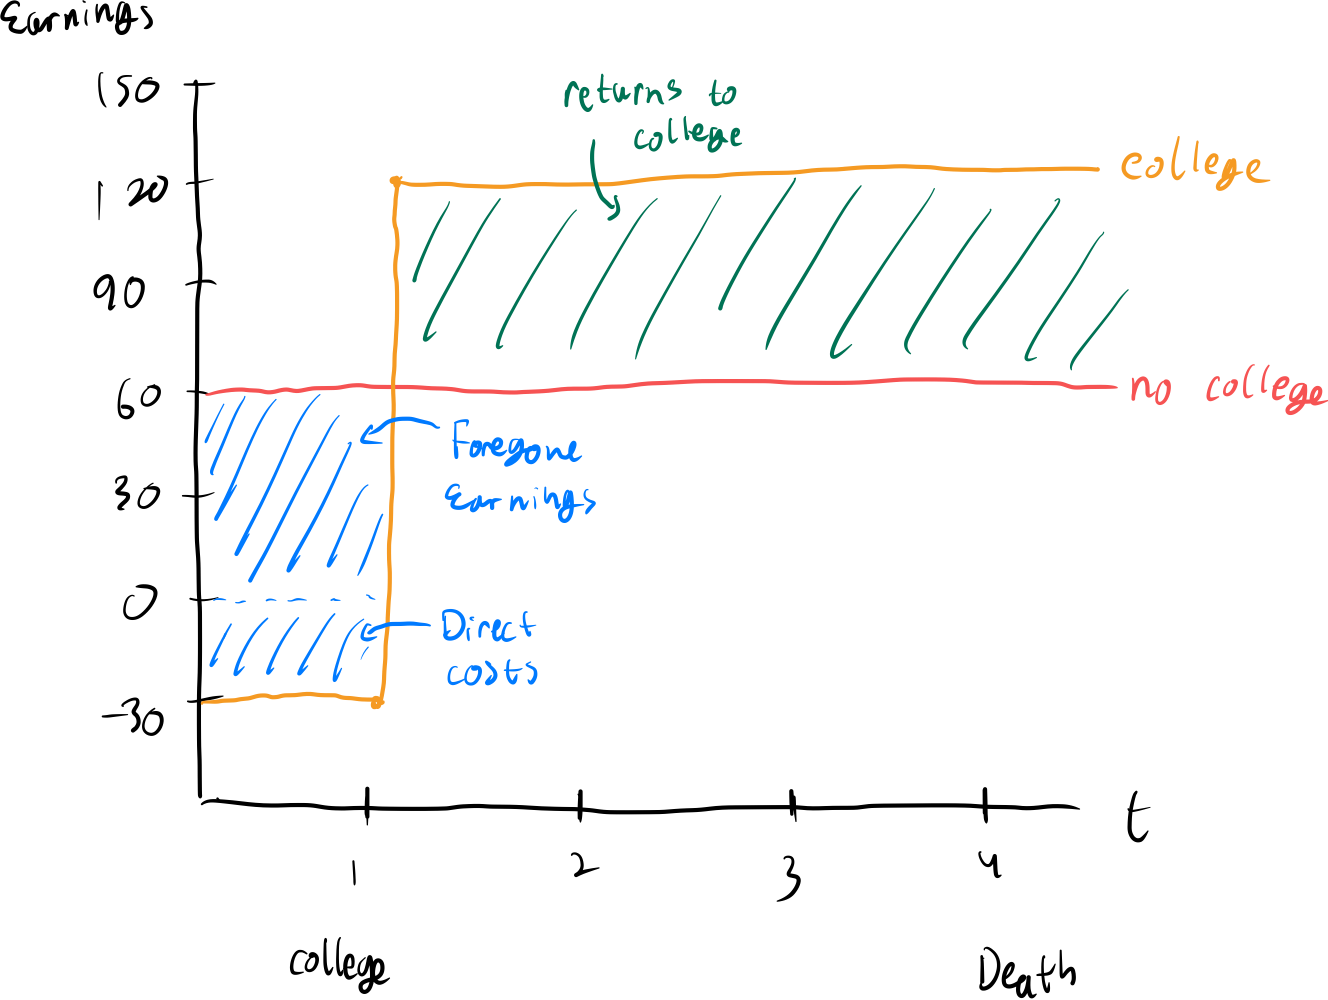
\includegraphics[width=10cm]{images/discrete_education_model.png}
      \end{center}
      The discount rate of \$100 in $t>0$ periods is worth $\frac{100}{(1+r)^t}$ in period $0$ (aka today).\\

      We generally think about $r$ in terms of the interest rate --- money today is worth more than money in the future due to the ability to invest.\\

      The \textit{present value} of a stream of money is found as follows:
      \begin{align*}
        \text{PV} &= \frac{100}{(1+r)} + \frac{100}{(1+r)^2} + \cdots + \frac{100}{(1+r)^n}\\
                  &= \sum_{t=1}^{n} \frac{100}{(1+r)^t} \tag*{$(1)$}\\
        (1+r)\text{PV} &= 100 + \frac{100}{(1+r)} + \cdots + \frac{100}{(1+r)^{n-1}}\\
                       &= 100 + \sum_{t=1}^{n-1} \frac{100}{(1+r)^t} \tag*{$(2)$}\\
        (1+r)\text{PV} - \text{PV} &= 100 + \sum_{t=1}^{n-1}\frac{100}{(1+r)^t} - \sum_{t=1}^{n-1}\frac{100}{(1+r)^t} - \frac{100}{(1+r)^n}\tag*{$(2)-(1)$}\\
        r\text{PV} &= 100 - \frac{100}{(1+r)^n}\\
        \text{PV} &= \frac{100}{r}\left(1-\frac{100}{(1+r)^n}\right)
      \end{align*}
      As $n$ becomes larger, then the PV of the asset is larger. For example, if $n = 40$, $Y = 60,000$, and $r = 0.05$, then the PV of this revenue stream is approximately \$1 million.\\

      Bringing this to the model, where $F$ denotes direct tuition cost, $Y_0$ denotes earnings with no schooling, and $Y_S$ denotes earnings with schooling (where school occurs in period $1$).
      \begin{align*}
        \text{PV}_{0} &= \frac{Y_0}{(1+r)} + \frac{Y_0}{(1+r)^2} + \cdots + \frac{Y_0}{(1+r)^n}\\
        \text{PV}_{S} &= -F + \frac{Y_S}{(1+r)^2} + \cdots + \frac{Y_S}{(1+r)^n}\\
        \text{NPV}_{S} &= \text{PV}_{S} - \text{PV}_{0}\\
                       &= \underbrace{-F - \frac{Y_0}{(1+r)}}_{\small\text{Cost}} + \underbrace{\sum_{t=2}^{n}\frac{Y_S - Y_0}{(1+r)^t}}_{\small\text{Benefit}}\\
                       &= -F-\frac{Y_0}{1+r} + \frac{Y_S-Y_0}{r}\left(1-\frac{1}{(1+r)}\right)\frac{1}{1+r}
      \end{align*}
      To find if education is worth it, we calculate if $\text{NPV}_{S} > 0$.
    \item[Continuous Model (or Mincer Model):] To take an extra year of education or not?
      \begin{itemize}
        \item $S$ is a discrete, integer choice (denoting a year of education).
        \item $Y_S$ is salary after schooling for $S$ years.
        \item There are zero direct costs of school.
        \item Years in labor force, $K$, are equivalent regardless of $S$.
      \end{itemize}
      We choose $S$ where marginal benefit is equal to marginal cost.
      \begin{align*}
        \text{PV}_{S} &= \text{PV}_{S+1}\\
        \sum_{t=1}^{K}\frac{Y_S}{(1+r)^t} &= \sum_{t=2}^{K+1}\frac{Y_{S+1}}{(1+r)^t}\\
        \frac{Y_S}{r}\left(1-\frac{1}{(1+r)^K}\right) &= \frac{Y_{S+1}}{r}\left(1-\frac{1}{(1+r)^K}\right)\frac{1}{1+r}\\
        Y_S &= Y_{S+1}\frac{1}{1+r}\\
        1+r &= \frac{Y_{S+1}}{Y_S}
      \end{align*}
      We choose school until the marginal rate of return is equal to the discount rate.
  \end{description}
  \textbf{Housekeeping, January 30:} Schedule for discussion and presentation is located \href{https://docs.google.com/document/d/1uy96HLNuZVGlrT8oiC49i3M6p2E57fopxGwizHv4_Hs/edit}{at this link}, and the guidelines for classroom activities are located \href{https://docs.google.com/document/d/1tnPmI21LJLdKblCUbuFMuDGobuAz2IOaineH_I4BTFg/edit}{at this link}.
  \subsection{Educational Landscape}%
  The human capital system consists of a number of components.
  \begin{itemize}
    \item Trade, technical, and vocational education (generally falls under post-secondary education)
    \item Early childhood education --- Ages 6 weeks--5, includes day care and pre-K
    \item Primary education --- Ages 5--12, Grades K--5/6
    \item Secondary education --- Ages 12--18, Grades 6--12
    \item Post-secondary education --- two year/community college, four year college
    \item Graduate education --- profession-oriented (MBA, JD), research-oriented (master's, PhD), certification (CPA, CFA, actuarial credentialing)
    \item Adult education (GED, college)
  \end{itemize}
  In primary and secondary education, primary choice facing consumers of education is between public and private education.
  \subsection{Human Capital Model: Choice of Schooling Quantity}%
  The human capital model indicates that consumers of education choose their amount of schooling, $S$, based on the following factors:
  \begin{itemize}
    \item Discrete: $Y_S$ (income from having been schooled) vs $Y_0$ (income without schooling)
    \item Continuous: $\frac{Y_{S+1}}{Y_S}$ (marginal rate of return from schooling)
    \item $F$ (the cost of schooling)
    \item $r$ (discount rate)
  \end{itemize}
  However, this leads us to ask an important question --- why might $S$ differ?
  \begin{itemize}
    \item Differing (marginal) rates of return --- job-specific factors, overqualification, ability, quality of education
    \item Different cost of education --- borrowing, aid, credit constraints
      \begin{description}
        \small
        \item[Comment:] Credit constraints increase exponentially as quantity of schooling increases.
      \end{description}
  \end{itemize}
  A model of credit constraints' effects on choices of education can be seen as follows:
  \begin{center}
    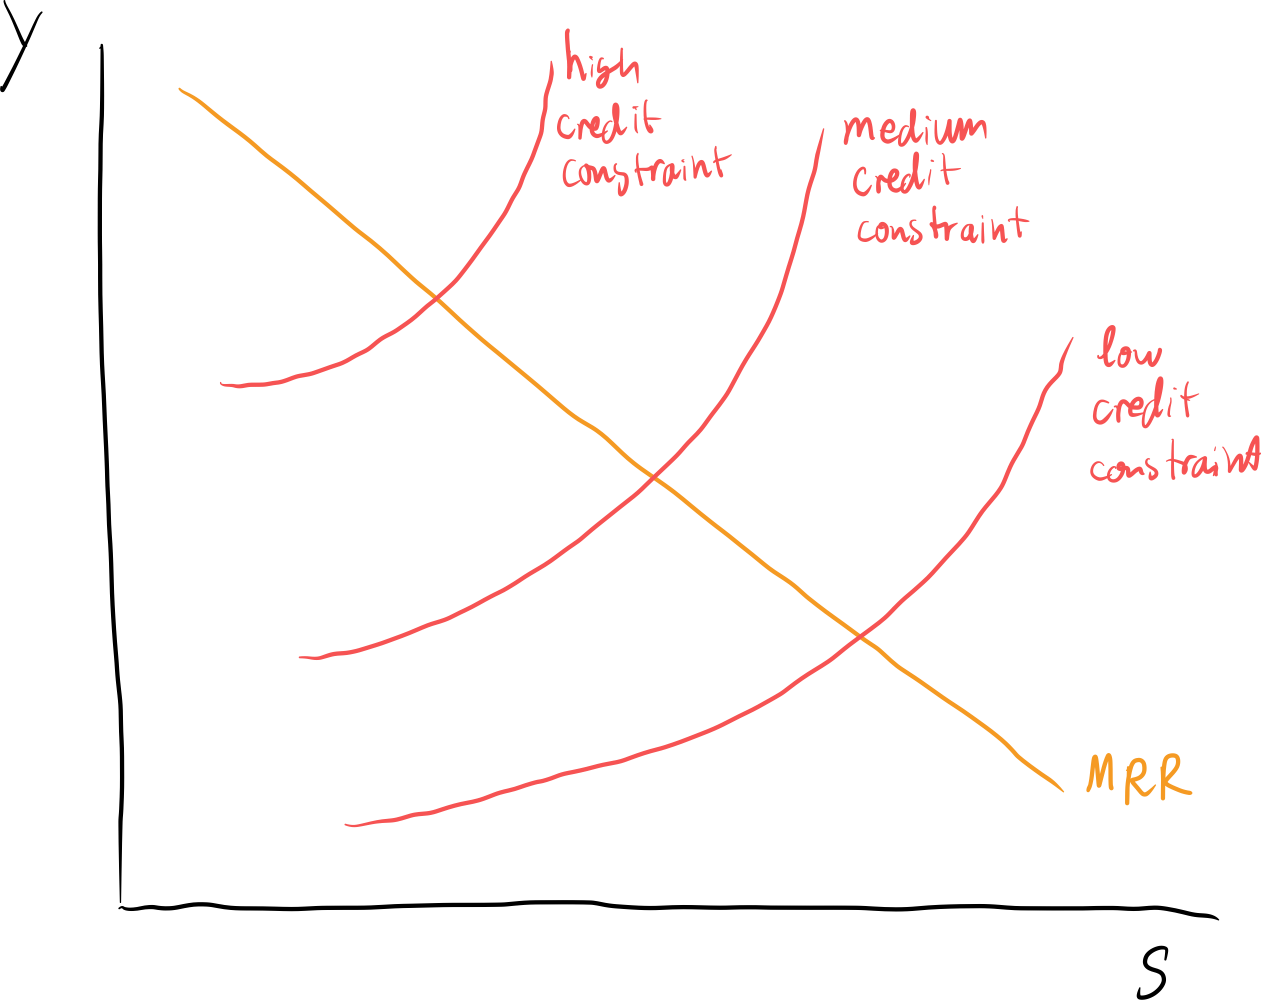
\includegraphics[width=10cm]{images/credit_constraints.png}
  \end{center}
  Broadly speaking, if $S$ differs because of marginal rate of return, then subsidies may be inefficient --- subsidies will cause inefficient excess schooling.\\

  However, if $S$ differs because of cost, then subsidies improve overall output and efficiency.
  \subsection{Signaling}%
  The basic idea behind the human capital model is that by getting more educated, you become smarter and have a higher rate of return --- regardless of whether or not you get a degree. Now, we will discuss a model where schooling does not indicate one's level of smartness.
  \begin{description}
    \item[Assumptions:]\hfill
      \begin{enumerate}[(1)]
        \item No human capital accrued at school.
        \item Two types of workers: low ability ($L$) of proportion $p$ with productivity $1$ and high ability ($H$) of $1-p$ with productivity $2$.
        \item Cost of education is lower for type $H$. For type $L$, the cost of education is $c$, and for type $H$ the cost of education is $c/2$.
        \item Generic employer who, if they distinguish $H$ and $L$, pay marginal benefit --- wage to $L$ is $1$, wage to $H$ is $2$.
        \item If the employer cannot distinguish between $H$ and $L$, then they pay the expected marginal benefit, $(1-p)(2) + (p)(1) = 2-p$.
      \end{enumerate}
    \item[Game Play:] \hfill
      \begin{itemize}
        \item Employer forms belief $w(S)$ about the worker productivity
        \item Employer sets $w(S)$
        \item Workers observe $w(S)$ and decide on $S$
        \item Workers are hired and firms observe their productivity
      \end{itemize}
    \item[Types of Equilibria:]\hfill
      \begin{itemize}
        \item Separating equilibrium: a situation where $H$ chooses education and $L$ does not choose education. In this case, education serves as a pure signal of high productivity --- there is no separating equilibrium where $H$ chooses no education and $L$ chooses education.
        \item Pooling equilibrium: all workers choose education, and the employer cannot differentiate, meaning the employer pays $2-p$ to all workers.
      \end{itemize}
    \item[Finding a Separating Equilibrium:] We assume that there is a separating equilibrium --- $H$ chooses $S=1$ and $L$ chooses $S=0$. Then, the employer forms beliefs to set a wage structure as follows:
      \begin{align*}
        w(S) &= \begin{cases}
          2 & S=1\\
          1 & S=0
        \end{cases}.
      \end{align*}
      In order to be an equilibrium, both $H$ and $L$ types need to have an incentive not to deviate.
      \begin{itemize}
        \item $H$ Type Equilibrium Condition: Return to education is higher than return to non-education.
          \begin{align*}
            2 - \frac{c}{2} &> 1\\
            c &< 2
          \end{align*}
        \item $L$ Type Equilibrium Condition: Return to non-education is higher than return to education.
          \begin{align*}
            1 &> 2-c\\
            c &> 1
          \end{align*}
      \end{itemize}
      Therefore, if $c\in (1,2)$, we can find a separating equilibrium.
    \item[Finding a Pooling Equilibrium:] We assume that there is a pooling equilibrium where all players are educated --- $H$ chooses $S = 1$ and $L$ chooses $S = 1$. Then, the employer forms beliefs to set a wage structure as follows:
      \begin{align*}
        w(S) &= \begin{cases}
          2-p & S = 1\\
          1 & S = 0
        \end{cases}
      \end{align*}
      In order to be an equilibrium, both $H$ and $L$ types need to have an incentive not to deviate.
      \begin{itemize}
        \item $H$ type equilibrium Condition: Return to education is higher than return to non-education.
          \begin{align*}
            (2-p)-\frac{c}{2} &> 1\\
            c &< 2-2p
          \end{align*}
        \item $L$ type equilibrium condition: Return to education is higher than return to non-education.
          \begin{align*}
            (2-p)-c &> 1\\
            c &< 1-p
          \end{align*}
      \end{itemize}
      Therefore, so long as $c < 1-p$, both types of employees will choose education over non-education. Essentially, if the cost of education is very low, then everyone will choose education.\\

      Working through a similar set of logic, we can also find a sufficient $c$ such that everyone chooses no education.
      \begin{align*}
        w(S) &= \begin{cases}
          2-p & S=0\\
          2 & S=1
        \end{cases},
      \end{align*}
       if $c > 2p $. Notice that both of these pooling equilibria are more likely to exist the higher proportion of $H$ types.
  \end{description}
  \subsubsection{Signal vs Index}%
  \begin{itemize}
    \item Signal: implicit assurance of skill or quality, chosen by worker, not readily apparent. Examples include education levels.
    \item Index: worker cannot control said assurance of skill or quality, but predetermined, generally a source of discrimination. Examples include disability, race, gender, and age.
  \end{itemize}
  The signaling model starts with employers offering different wages based on a signal --- the signal is something a worker has some level of control.\\

  However, the signaling model could also be thought of as an indexing model (by varying parameters $p$ and $c$ while equalizing productivity). Essentially, the signaling model is about a legal form of discrimination (education-based discrimination), but we can apply it to illegal forms of discrimination.
  \subsection{Human Capital and Signaling Model: Features}%
  \begin{center}
    \renewcommand{\arraystretch}{1.5}
    \begin{tabular}{m{0.2\textwidth}|m{0.2\textwidth}|m{0.2\textwidth}}
      Human Capital & Both Models & Signaling Model\\
      \hline
      positive externalities & inequality & pure private returns\\
      education is efficient & & education is inefficient
    \end{tabular}
  \end{center}
  \section{Claudia Goldin: The Human-Capital Century}%
  \begin{itemize}
    \item The 20th century was the century where people became educated --- early on, few people even had a primary education, but now, the vast majority of people obtain secondary school.
    \item Education is democratic.
      \begin{itemize}
        \item Democracy is a government by the people, for the people.
        \item Power is not vested by God or inherent in blood, but governance comes from the consent of the governed.
        \item Public demand for education leads to more education being delivered.
        \item Education provides both skills and time to create better citizens.
      \end{itemize}
    \item Virtues: egalitarianism, forgiveness (possibly changing), separation of church and state.
    \item Primary education was very common across the rich world, but secondary education was far more common in the United States than other countries.
    \item Specifically, American secondary education was about \textit{general} education (algebra, writing, reading comprehension, etc.), not merely vocational or technical training. The European system is much more heavily tracked.
    \item Idea that one would spend years 10--18 in education began in the United States. Adults were better able to establish themselves in the new economy, and the underlying structures were exported to the rest of the United States.
    \item European systems developed out of monarchy/aristocracy, leading to deterministic ideas of the demands of the economy.
    \item Decentralized American education system --- curriculum followed the economy, rather than determined for the economy.
    \item The standards for general education developed around a pure method of approach towards problems.
    \item Rise of large corporations generated large need for management, idea generation, communication --- had to do HR, accounting, etc. at a scale never seen before. Skills were meant to be portable and transferable, which the decentralized American education system satisfied the demand for.
  \end{itemize}
  \section{Understanding Causality}%
  When discussing questions in economics, there are two basic approaches:
  \begin{itemize}
    \item Theory: models (as discussed in our model of human capital and the signaling model).
    \item Empirics: using data to understand the dynamics of the world.
  \end{itemize}
  For example, we may want to understand the impact of a good teacher in the role of educational success through different measures:
  \begin{itemize}
    \item Pass rates or graduation rates.
    \item College entrance rates.
    \item Test scores.
    \item Earnings.
  \end{itemize}
  We can think of each of these as our $Y_i$, our outcome variable of interest. At the same time, we have to measure the quality of a teacher, $X_i$, through different mechanisms:
  \begin{itemize}
    \item Education
    \item Course Evaluations (with adequate controls for race and gender)
    \item Subject
  \end{itemize}
  \subsection{Defining Causality}%
  The impact of variable $A$ \textit{causally} affects variable $B$ as the change in $B$ if $A$, and only $A$, is altered. Causality is usually defined using a counterfactual.\\

  In the case of education, for $Y_i$, student $i$'s outcome, with $Y_{1i}$ for an outcome for a student with a good teacher and $Y_{0i}$ for a student with a bad teacher. We define $D_i$, our dummy variable, as $1$ if the teacher is good and $0$ if the teacher is bad.
  \begin{align*}
    Y_i &= Y_{0i} + D_i\underbrace{(Y_{1i} - Y_{0i})}_{\text{treatment effect}}.
  \end{align*}
  \subsection{Potential Outcomes Framework}%
  \begin{itemize}
    \item What does a researcher observe? We assume $N>1$. In this case, 
  \end{itemize}
  \begin{align*}
    E(Y_{1i}|D_i=1) - E(Y_{0i}|D_i=0) &= \text{ observed difference of $D_i = 1$ }\\
                                      &= \overbrace{E(Y_{1i}|D_i = 1) - \underbrace{E(Y_{0i}|D_i=1)}_{\text{counterfactual}}}^{\text{Average Treatment Effect (impact of good teacher)}}\\
                                      &+ \overbrace{\underbrace{E(Y_{0i}|D_i=1)}_{\text{counterfactual}} - E(Y_{0i}|D_i=0)}^{\text{selection bias}}
  \end{align*}
  Therefore, we can see that the observed difference is a function of treatment and selection bias. The most difficult part of empirical research is finding situations where selection bias is as close to zero as possible.\\

  In regression analysis, we might have the model that states
  \begin{align*}
    \text{score}_i &= \beta_0 + \beta_1\text{TeacherQuality}_i + \varepsilon_i.
  \end{align*}
  \begin{center}
    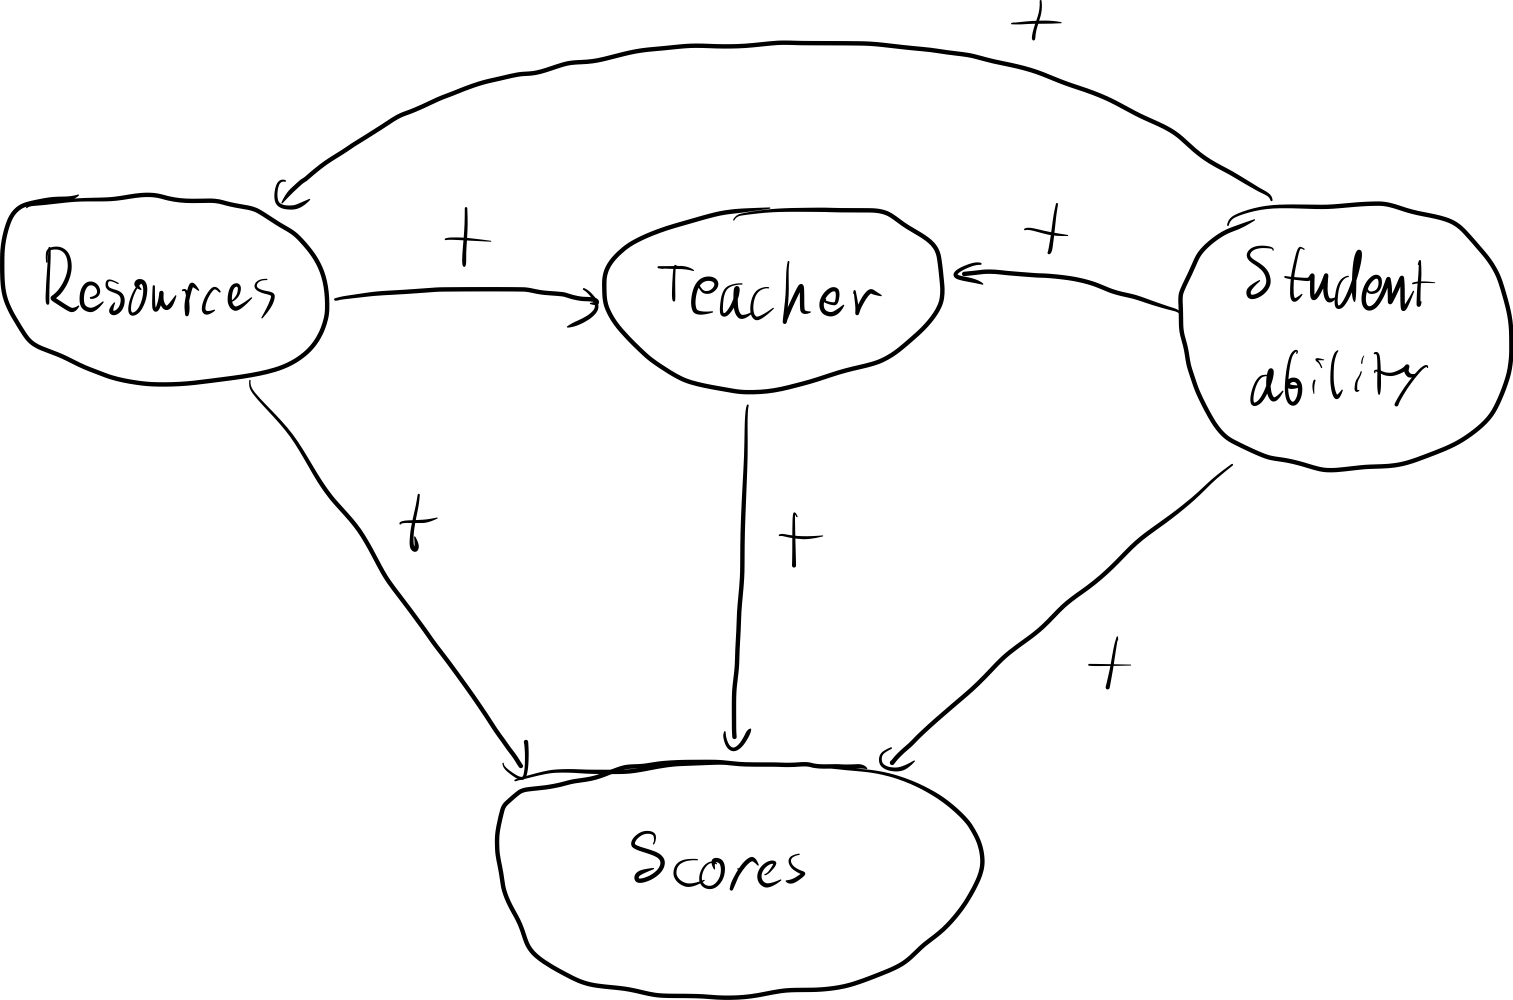
\includegraphics[width=10cm]{images/test_score_variables.png}
  \end{center}
  Suppose that teachers matter --- even then, there are other variables, such as resources or intrinsic ability. The diagram depicts the various ways that selection bias can create positive correlation.\\

  In this case, $\hat{\beta_1}$ will be biased by selection. This is known as omitted variable bias, and violates the principle that $\text{Cov}(X,\varepsilon) = 0$.\\

  To resolve this, we may update our regression model to control for the omitted variable of resources, denoted $Z$.
  \begin{align*}
    \text{score}_{i} &= \beta_0 + \beta_1\text{TeacherQuality}_i + \beta_2\text{Resources}_i + \varepsilon_i\\
    \text{observed effect} &= E(Y_{1i}|D_i=1,Z) - E(Y_{0i}|D_{i}=1,Z) + \underbrace{E(Y_{0i}|D_i=1,Z) - E(Y_{0i}|D_i=0,Z)}_{\text{selection bias}}.
  \end{align*}
  However this still leaves out other omitted variables (such as parental involvement). As we add more control variables, selection bias should reduce. All these control variables exist to mitigate selection bias and make a non-experimental setting as close to an experiment as possible.\\

  There are a few major ways to identify causality:
  \begin{enumerate}[(1)]
    \item Experiments
    \item Instrumental Variables
    \item Difference-in-difference
    \item Regression discontinuity
    \item Panel data
  \end{enumerate}
  \subsection{Experiments}%
  The ``cleanest'' way to 
  \begin{itemize}
    \item Identify a Target Population.
    \item Randomize Population.
      \begin{itemize}
        \item Treatment group experiences condition.
        \item Control group does not experience condition.
      \end{itemize}
    \item Experiments have the following desirable properties:
      \begin{itemize}
        \item Internal Validity: $E(\varepsilon|X) = 0$ (error is uncorrelated with independent variable)
        \item Randomness
      \end{itemize}
    \item However, true randomness is difficult to attain. The ABCs of experiments also threaten internal validity.
      \begin{itemize}
        \item Attrition: individuals drop out of experiments.
        \item Balance: distribution of covariates may not be the same across groups.
        \item Compliance: not everyone assigned to a treatment may experience it.
      \end{itemize}
    \item There are also other limits:
      \begin{itemize}
        \item Feasibility: expense, time, or even full impossibility.
        \item Ethics: some experiments may pose ethical issues
        \item External validity: experiments may only provide insights to specific situations.
      \end{itemize}
    \item Threats to internal validity:
      \begin{itemize}
        \item Poor randomization
        \item Experimental contamination
        \item Response rate, compliance
        \item Attrition
      \end{itemize}
    \item Threats to external validity:
      \begin{itemize}
        \item Non-representative sample
        \item Treatment depends on experiment
        \item Excessive controls, Hawthorne effect
        \item Scalability
      \end{itemize}
  \end{itemize}
\end{document}
